\begin{figure}
    \begin{center}
        % 
\includegraphics[width=0.5\textwidth]{papers/particles/figures/wavesim/particle_initial_state.png}
        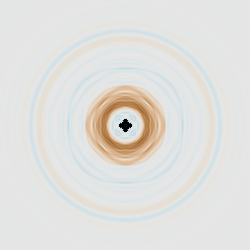
\includegraphics[width=0.5\textwidth]{papers/particles/figures/simulations/particle_frames/frame_02.png}
        % Alternative 1: 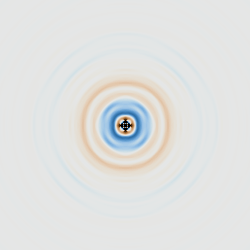
\includegraphics[width=0.5\textwidth]{papers/particles/figures/simulations/particle_frames/frame_04.png}
        \caption{Feldkonfigurationen mit zunehmend wachsender Energieansammlung im Zentrum der Simulation.\ \mytodo{Bild anpassen}}\label{particles:fig:partikel:wachsen}
    \end{center}
\end{figure}